\documentclass{standalone}
\usepackage{tikz}
\usepackage{ctex,siunitx}
\setCJKmainfont{Noto Serif CJK SC}
\usepackage{tkz-euclide}
\usepackage{amsmath}
\usetikzlibrary{patterns, calc,3d}
\usetikzlibrary {decorations.pathmorphing,decorations.pathreplacing,decorations.shapes}
\begin{document}
\small
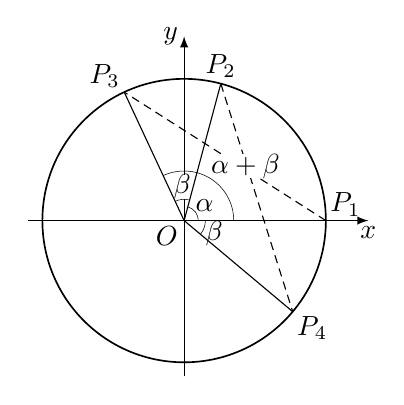
\begin{tikzpicture}[>=latex,scale=0.9,inner sep=0pt]
  \draw[->](0,-2.2)--(0,2.6)node[left=2pt]{$y$};
  \draw[very thin](0.2,0)arc(0:75:0.2)node[midway,above right]{$\alpha$};
  \draw[very thin](0.3,0)arc(0:-40:0.3)node[at start,below right]{$\beta$};
  \draw[very thin](75:0.3)arc(75:115:0.3)node[midway,above,fill=white]{$\beta$};
  \draw[->](-2.2,0)--(2.6,0)node[below=2pt]{$x$};
  \node at (0,0)[below left=3pt]{$O$};
  \draw[semithick](0,0)circle(2);
  \node at (2,0)[above right=2pt]{$P_1$};
  \draw(0,0)--(115:2)node[above left=2pt]{$P_3$};
  \draw(0,0)--(75:2)node[above=2pt]{$P_2$};
  \draw(0,0)--(-40:2)node[below right=2pt]{$P_4$};
  \draw[densely dashed](2,0)--(115:2);
  \draw[densely dashed](75:2)--(-40:2);
  \draw[very thin](0.7,0)arc(0:115:0.7)node[midway,above right,fill=white]{$\alpha+\beta$};
\end{tikzpicture}
\end{document}